%% 
%% Copyright 2007, 2008, 2009 Elsevier Ltd
%% 
%% This file is part of the 'Elsarticle Bundle'.
%% ---------------------------------------------
%% 
%% It may be distributed under the conditions of the LaTeX Project Public
%% License, either version 1.2 of this license or (at your option) any
%% later version.  The latest version of this license is in
%%    http://www.latex-project.org/lppl.txt
%% and version 1.2 or later is part of all distributions of LaTeX
%% version 1999/12/01 or later.
%% 
%% The list of all files belonging to the 'Elsarticle Bundle' is
%% given in the file `manifest.txt'.
%% 

%% Template article for Elsevier's document class `elsarticle'
%% with numbered style bibliographic references
%% SP 2008/03/01

\documentclass[preprint,12pt]{elsarticle}

%% Use the option review to obtain double line spacing
%% \documentclass[authoryear,preprint,review,12pt]{elsarticle}

%% Use the options 1p,twocolumn; 3p; 3p,twocolumn; 5p; or 5p,twocolumn
%% for a journal layout:
%% \documentclass[final,1p,times]{elsarticle}
%% \documentclass[final,1p,times,twocolumn]{elsarticle}
%% \documentclass[final,3p,times]{elsarticle}
%% \documentclass[final,3p,times,twocolumn]{elsarticle}
%% \documentclass[final,5p,times]{elsarticle}
%% \documentclass[final,5p,times,twocolumn]{elsarticle}

%% For including figures, graphicx.sty has been loaded in
%% elsarticle.cls. If you prefer to use the old commands
%% please give \usepackage{epsfig}

%% The amssymb package provides various useful mathematical symbols
\usepackage{amssymb}
\usepackage{booktabs}
\usepackage{amsmath}
\usepackage{algorithm}
\usepackage{lscape}
\usepackage[noend]{algpseudocode}

%% The amsthm package provides extended theorem environments
%% \usepackage{amsthm}

%% The lineno packages adds line numbers. Start line numbering with
%% \begin{linenumbers}, end it with \end{linenumbers}. Or switch it on
%% for the whole article with \linenumbers.
%% \usepackage{lineno}
\journal{Nuclear Physics B}
\bibliographystyle{elsarticle-num}
\begin{document}

\begin{frontmatter}

%% Title, authors and addresses

%% use the tnoteref command within \title for footnotes;
%% use the tnotetext command for theassociated footnote;
%% use the fnref command within \author or \address for footnotes;
%% use the fntext command for theassociated footnote;
%% use the corref command within \author for corresponding author footnotes;
%% use the cortext command for theassociated footnote;
%% use the ead command for the email address,
%% and the form \ead[url] for the home page:
%% \title{Title\tnoteref{label1}}
%% \tnotetext[label1]{}
%% \author{Name\corref{cor1}\fnref{label2}}
%% \ead{email address}
%% \ead[url]{home page}
%% \fntext[label2]{}
%% \cortext[cor1]{}
%% \address{Address\fnref{label3}}
%% \fntext[label3]{}

\title{Optimized and Cost Considering Huffman Code For Biological Data Transmission}

%% use optional labels to link authors explicitly to addresses:
%% \author[label1,label2]{}
%% \address[label1]{}
%% \address[label2]{}

\author{}

\address{}

\begin{abstract}
%% Text of abstract

\end{abstract}

\begin{keyword}
%% keywords here, in the form: keyword \sep keyword

%% PACS codes here, in the form: \PACS code \sep code

%% MSC codes here, in the form: \MSC code \sep code
%% or \MSC[2008] code \sep code (2000 is the default)

\end{keyword}

\end{frontmatter}

%% \linenumbers

%% main text
\section{Introduction}
\section{Background}
\subsection{Issues on Biological Data Transmission}
The size of biological data including DNA sequences increase with an ever expanding rate and will be bigger and bigger in the future. These Biological data are stored in biology database, the exponential growth of these database become a big problem to all biological data processing methods.
Different operation will be applied to these data such as, searching [],e-mail attachment [], alignment [], and transmission on distributed computing []. Interestingly, biological data compression can play a key role in all biological data processing.\\  
A recent deluge of interest in the development of new tools for biological data processing, these all algorithms needs an efficient methods for data compression. The main objective of data compression methods is minimizing the number of bits in the data representation. 
In [Marty C. Brandon ] authors propose a new general data structure and data encoding approach for the efficient storage of genomic data. This method encode only the differences between a genome sequence and a reference sequence, the method use different encoding scheme from fixed codes such as Golomb and Elias codes, to variables codes, such as Huffman codes. Other methods based on same idea to encode only the difference between reference sequence and the target one, Authors in [Scott Christley1] uses Huffman code for encoding difference between sequence to sent it as an email attachment, but these methods suffer that they must sent the reference sequence for at least one time for each species.\\
Wang and Zhang (2011) proposed a new scheme for referential compression of genomes based on the chromosome level. The Algorithm aim to search for longest common subsequence between matching parts and the differences encoded using Huffman coding.\\
All previous studies focus only on the differences and the relation between continuation of the sequence, and without improvement of the encoding scheme.
\subsection{Rationale of Unequal Bit Cost Considering Encoding Approaches}
In the recent years, application of battery-powered portable devices, e.g. laptop computers and mobile phones has increased significantly. Proper representation of digital data and their transmission efficiency has become a primary concern for digital community because it affects the performance, reliability, and the cost of computation in both portable and non-portable devices. CMOS technologies were developed in order to reduce the power consumption both in data processing and transmission. In order to increase transmission speed and reduce transmission cost, parallel data transmission methods are widely used. However, parallel transmission is limited to short distance communications, e.g. locally connected devices, internal buses. Ruling out the possible availability of parallel transmission
links over long distance, we are left with its serial alternative only. 

Data encoding techniques came into action to improve the data transmission efficiency over serial communication medium by compressing data before transmitting. Efficiency can be measured in terms of incurred cost, required storage space, consumed power, time spent and likewise. Data must be
encoded to meet the purposes like: unambiguous retrieval of information, efficient storage, efficient transmission and etc. Let a message consist of sequences of characters taken from an alphabet $\Sigma$, where  $\alpha_1,\alpha_2,\alpha_3\ldots,\alpha_r$ are the elements that represent the characters in the source $\Sigma$. The length of $\alpha_i$ represents its cost or transmission time, i.e., $c\left(\alpha_i\right)= length(\alpha_i)$. A codeword $w_i$ is a string of characters in $\Sigma$, i.e., $w_i\in\Sigma^{+}$. If a codeword is $w_i=\alpha_{i1},\alpha_{i2},\ldots,\alpha_{in}$, then the length or cost of the codeword is the sum of the lengths of its constituent elements:

\begin{equation}
\label{eqn1}
  \text{cost}\left(w_i\right)=\sum_{j=1}^{n}c\left(\alpha_{ij}\right)
\end{equation} 
  
If all the elements of a codeword has unit cost or length then the cost of the codeword is equivalent to the length of the codeword. However, it is not necessary for the elements in the codeword to have equal length or cost. For example, in Morse Code all the ASCII characters are encoded as sequence of dots ($\cdot$) and dashes($-$) where a dash is three times longer than a dot in duration \cite{Redmond09}. However, the Morse code scheme suffers from the prefix problem \cite{Gr03}. Ignoring the prefix problem, Morse Code results in a tremendous savings of bits over ASCII representation. Using Morse Code, we can treat the binary bits differently; 0 as a dot and 1 as a dash. Even if we consider the voltage level to represent the binary digits then they are still different. Table \ref{table1} shows the logic level to represent binary digits in CMOS and TTL technologies. 

\begin{table}[thpb]
\renewcommand{\arraystretch}{1.5}
\caption{Example of binary logic level}
\label{table1}
\centering
\begin{tabular}{c c c c}
\hline
 \bfseries Technology  & 0 & 1&Notes\\
\hline
\bfseries CMOS & $0~V$ to $\frac{V_{DD}}{2}$&$\frac{V_{DD}}{2}$ to $V_{DD}$&$V_{DD}$= supply voltage\\
%\hline
\bfseries TTL & $0~V$ to $0.8~V$&$2~V$ to $V_{CC}$ &$V_{CC}$ is $4.75~V$ to $5.25~V$\\
%\hline
\hline
\end{tabular}
\end{table}

As the unequal letter cost problem is not new therefore it has been addressed by different researchers. The more general case where the costs of the letters as well as the probabilities of the words are arbitrarily specified was treated in \cite{Karp61}. A number of other researchers have focused on uniform sources and developed algorithm for the unequal letter costs encoding \cite{Gil95, Kar62,Varn71,AltMel80,perl1975}.  Let $p_1,p_2,\ldots,p_n$ be the probabilities with which the source symbols occur in a message and the codewords representing the source symbols are $w_1,w_2,\ldots,w_n$ then the cost of the code $W$ is:

\begin{equation}
C\left(W\right)=\sum_{i=1}^{n}cost\left(w_i\right).p_i 
\end{equation}
The aim of producing an optimal code with unequal letter cost is to find a codeword $W$ that consists of $n$ prefix code letters each with minimum cost $c_i$ that produces the overall minimum cost $C\left(W\right)$, given that costs $0<c_1\leq c_2 \leq c_2 \ldots \leq c_n$, and probabilities $p_1\geq p_2\geq \ldots\geq p_n>0$.
%Digital CMOS circuits have three major sources of power dissipation and are summarised in the following equation \cite{Weste88}:
%\begin{equation}
%\begin{split}
%    P_{avg} ={}& P_{dynamic}+P_{short-circuit}+P_{leakage}\\
%         ={}& \alpha_{0 \rightarrow 1}\cdot C_L\cdot V_{dd}^2\cdot f_{clk} + I_{sc}\cdot V_{dd}+I_{leakage}\cdot V_{dd}
%\end{split}
%\end{equation}
\subsection{Huffman Codes}
In computer science and information theory, Huffman code is an entropy encoding algorithm used for lossless data compression. It takes into account the probabilities at which different symbols are likely to occur and results into fewer data bits on the average. 
%then assigns variable-length codes to different distinct symbols, and thus minimises the number of bits required to encode a message. 
For any given set of symbols and associated occurrence probabilities, there is an optimal encoding rule that minimises the number of bits needed to represent the source. Encoding symbols in predefined fixed length code, does not attain an optimum performance, because every character consumes equal number of bits irrespective to their degree of contribution to the whole message. Huffman code tackles this by generating variable length codes, given a probability usage frequency for a set of symbols. It generates prefix-code to facilitate unambiguous retrieval of information. A scheme of prefix code assigns codes to letters in $\Sigma$ to form codeword $w_i$ such that none of them is a prefix to another. For example, the codes $\left\{ 1,01,001,0001\right\}$ and $\left\{ 000,001,011,111\right\}$ are prefix-free, whereas the code $\left\{ 1,01,100\right\}$ is not, because 1 is a prefix in 100.

Applications of Huffman code are pervasive throughout
computer science. The algorithm to completely perform Huffman encoding and decoding is explained by \cite{Amst86}. It can be used effectively where there is a need for a compact code to represent a long series of a relatively small number of distinct bytes. For example, Table \ref{table1} shows 8 different ASCII characters, their frequencies, ASCII codes and the codewords generated for those symbols using Huffman code. It is seen from the table that the codeword to represent each character is compressed and the most frequent character gets the shortest code. In this example, the compression ratio obtained by Huffman code is 64.16\%.   

\begin{table}[thpb]
\renewcommand{\arraystretch}{1.3}
\caption{Example of application of Huffman Code to compress ASCII characters}
\label{table2}
\centering
\begin{tabular}{c c c c}
\hline
 Symbols & Frequency& ASCII Code &\begin{tabular}{@{}c@{}}Codewords using\\Huffman Code\end{tabular} \\
\hline
\bfseries A & 50&01000001&00\\
%\hline
\bfseries B & 35&01000010&101\\
%\hline
\bfseries C & 42&01000011&110\\
%\hline
\bfseries D & 22&01000100&1001\\
%\hline
\bfseries E & 65&01000101&01\\
%\hline
\bfseries F & 25&01000110&1111\\
%\hline
\bfseries G & 9&01000111&1000\\
%\hline
\bfseries H & 23&01001000&1110\\
\hline
\end{tabular}
\end{table}

\section{Approach}
\subsection{Proposed Scheme}
\begin{figure}[h]
\begin{center}
\caption{The proposed Scheme}
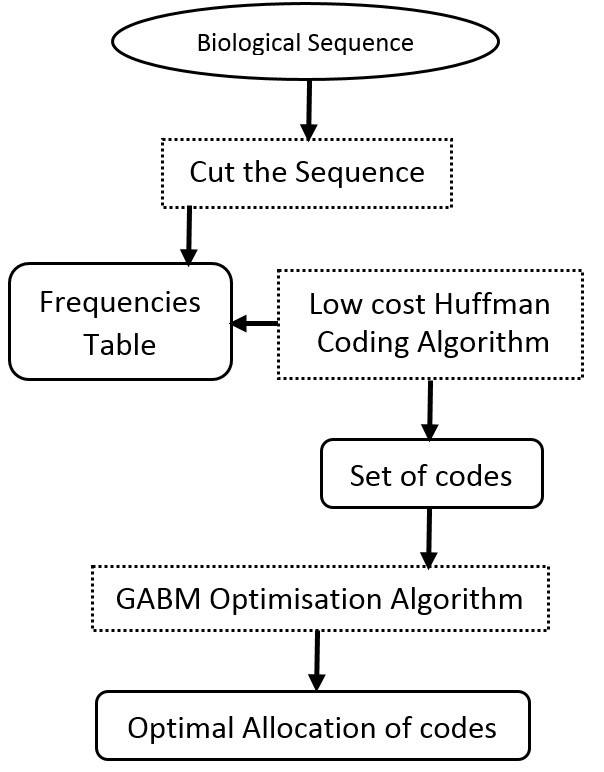
\includegraphics[scale=0.5]{Images/Drawing3.jpg}
\end{center}
\label{Fig1}
\end{figure}
\subsection{Power Efficient Huffman code}
\subsection{Optimisation of the Codes}
\subsubsection{Problem formulation}
The problem of finding the best allocation of codes to each symbol can be   modelled as an Assignment Problems with Constraint, the problem is formulated as follows :\\\\
\textbf{Definition:} Given a set of codes $C=\left\{C_{1},C_{2}...C_{n}\right\}$, and a set of frequencies $C=\left\{Q_{1},Q_{2}...Q_{n}\right\}$. For each code we have the length of the code $|C_{i}|$ (number of bits) and the cost of the code $S_{C_{i}}$ (cost of ones and zeros), the objective is to assign to each frequency a code in order to get the minimum total number of bits, while respecting the initial assignment total cost $S_{t}$.   
\\
The Objective Function is : 

\begin{equation}
Minimise \sum (|C_{i}| \times Q_{j}) 
\end{equation}
while :
\begin{equation}
\sum (|S_{C_{i}}| \times Q_{j}) \leqslant S_{t} 
\end{equation}
\subsubsection{Basic Genetic Algorithm}
Genetic Algorithm (GA) is a bio-inspired meta-heuristics algorithm developed by []. GA is a stochastic optimization algorithm imitate the natural evolution process of genomes. GA started by generate a population of random feasible solutions, the optimization process of GA is as follow, and we select two solution among the population, by one of the well-known selection techniques. This two selected solution will be considered as two parents, we generate two other new solutions from the two selected solution (Sons), this new solutions can be mutate according to a given mutation probability. The quality of each solution is computed with the fitness function which control the evolution of the GA population by the deletion of the worst solution and insertion of the good solutions among   parents and sons. This processes is repeated until the stopped criteria is achieved which can be the number of generation or if the population is stabilized.
\subsubsection{GA for Bits minimisation}
The main objective of the GA optimisation algorithm for bits minimisation (GaBm) problem is to assign to each frequency a specific code. The GaBm population is generated randomly from the different codes, and the affectation of codes to different frequencies given by the low cost considering  algorithm  to initial population to ensure that the final solution is better or at least equal to the solution given by the low cost considering Huffman code algorithm (step 1). The optimisation process of the genetic algorithms start with the selection of two solution randomly from the population (step 3). After that the operations of genetic algorithms are apply for the initial population optimization (see figure 3). Firstly the crossover operation are applied to these two selected  solution (considered as parents) to generate two new solutions (considered as sons)(step 4). These two children may contain conflict like finding a duplicated code allocated to two different frequencies in the solution, so a regulation step is done to ensure the correctness of the solution (see figure 3). Secondly these two new solutions are mutated according to a predefined probability (step 5), to ensure a good diversification on the space solutions. The next step is to add these two new solutions (children) to the population (step 6) (see figure 2). Finally the new population are ranked by fitness (step 7), and the worst solution are deleted until the initial size of the population are achieved  (step 8). the whole process are repeated until the max number of operation is achieved (step 9). 
\begin{algorithm}
\caption{GA for bits minimisation}
\begin{algorithmic}[1]
\State Population initialization (P).
\While {Max number of generation not achieved} 
\State Select two solutions $S_{1},S_{2}$ form P.
\State Crossover $S_{1},S_{2}$ to generate $S_{11},S_{21}$.
\State Mutate $S_{11},S_{21}$.
\State Add children to population
\State Rank the population by fitness
\State Remove worst candidates until population limit
\State Return to 2;
\EndWhile
\State Display the best solution from the population P;
\end{algorithmic}
\end{algorithm}

\begin{figure}[h]
\begin{center}
\caption{Population Update for genetic algorithm}
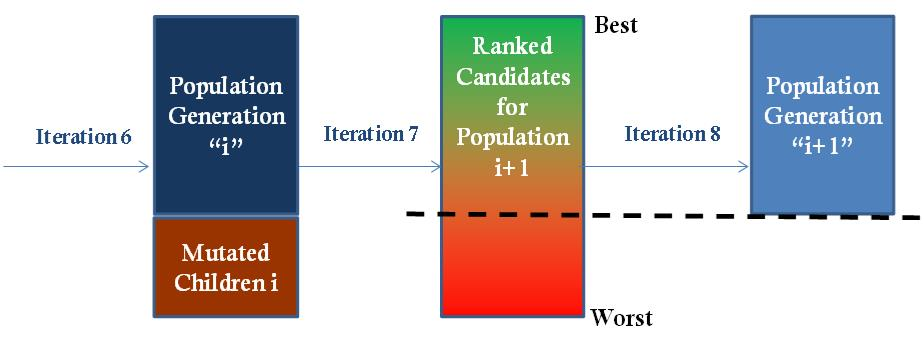
\includegraphics[scale=0.7]{Images/Drawing1.jpg}
\end{center}
\label{Fig1}
\end{figure}

\begin{figure}[h]
\begin{center}
\caption{Operations of genetic algorithm}
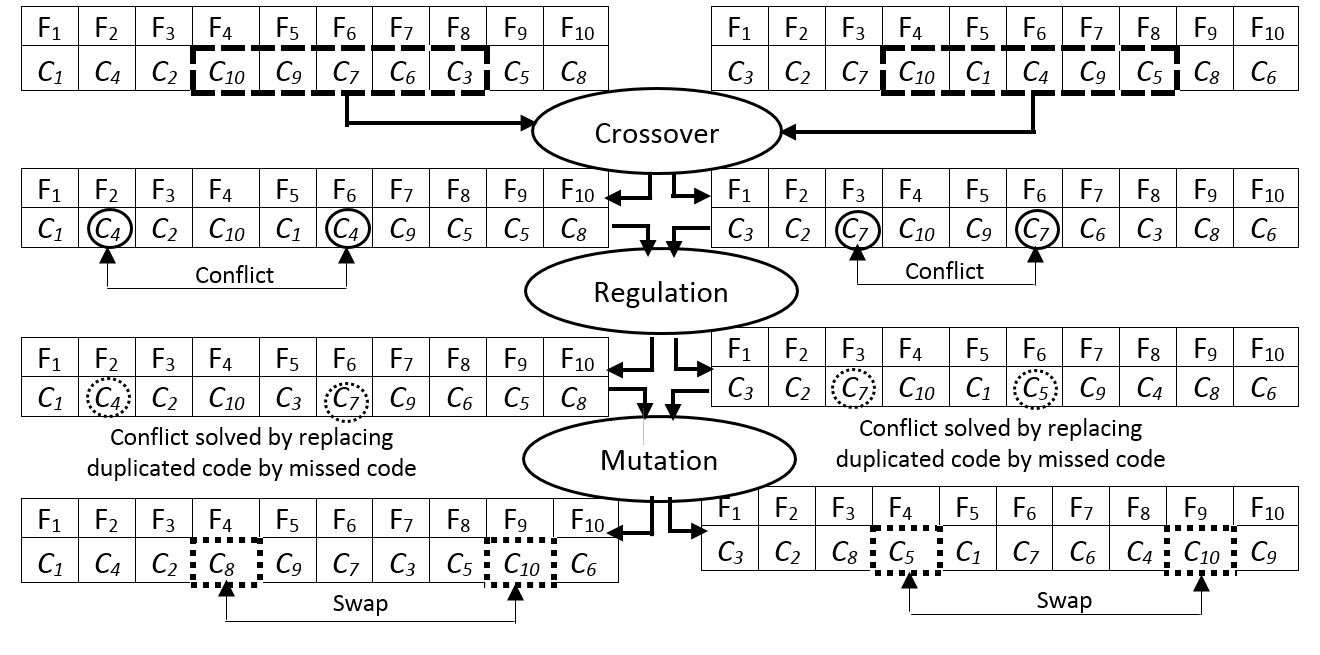
\includegraphics[scale=0.5]{Images/Drawing2.jpg}
\end{center}
\label{Fig1}
\end{figure}



\section{Results And Discussion}
\begin{landscape}
\begin{table*}
\small
\label{datas}
\caption{GABM for comparison for cost and number of bits of different approaches with different datasets}
\begin{center}
\begin{tabular}{c c c c c c c}
\toprule
$\textbf{Data sets}$ & \multicolumn{2}{c}{Huffman Algorithm} & \multicolumn{2}{c}{low cost considering  algorithm}& \multicolumn{2}{c}{Optimized algorithm}\\\hline
 & $\textbf{Cost}$	& $\textbf{Bits}$ &	$\textbf{Cost}$&	$\textbf{Bits	}$&$\textbf{Cost}$&	$\textbf{Bits}$
\\\hline
Mycobacterium smegmatis &76787151  &	37256819	&67272097	&41270715	&67272097&	40459089\\\hline
Amycolatopsis benzoatilytica &100425402&  	48778740	&88334137	&54602397	&88334137&	53281409\\\hline
Mycobacterium rhodesiae&75940155  	&36860555	&66629579	&40873035&	66629579&	40128089\\\hline
Streptomyces bottropensis&103552729  	&50047265	&90758205&	56109303&	90758205&	54281713\\\hline
Mycobacterium smegmatis. MC2&82234926  &	39772838	&71876260	&44199916&	71876260&	43338060\\\hline
Mycobacterium smegmatis MKD8&83454842  	&40370894	&72945595	&44805759	&72945595	&43945321\\\hline
Bradyrhizobium WSM471&92539488  &	44977876&	81176987&	49688369	&81176987	&49052869\\\hline
Amycolatopsis thermoflava&99613856 & 	48183688	&87033015&	53778627	&87033015&	52820213\\\hline
Bacillus thuringiensis serovar thuringiensis&71876739 &	34874617&	62637908&	38314532&	62637908&	37684296\\\hline
Bacillus thuringiensis Bt407&75324432 & 	36576034	&65658000&	40226924	&65658000&	39558890\\\hline
Pseudomonas aeruginosa 9BR&80766360  &	39092450&	70462778	&43020460&	70462778&	42260476\\\hline
Bacillus thuringiensis serovar berliner&74560825  &	36179579&	65001120	&39772574	&65001120&	39077012\\\hline
Bacillus thuringiensis serovar pakistani&71562941 & 	34737083	&62335103&	38118291&	62335103&	37629173\\\hline
Pseudomonas aeruginosa LES400&78261299 & 	37843793&	68212426&	41745748&	68212426&	40979588\\\hline
\bottomrule
\end{tabular}
\end{center}
\end{table*}
\end{landscape}

\section{Conclusion}



%% The Appendices part is started with the command \appendix;
%% appendix sections are then done as normal sections
%% \appendix

%% \section{}
%% \label{}

%% If you have bibdatabase file and want bibtex to generate the
%% bibitems, please use
%%
%%  \bibliographystyle{elsarticle-num} 
%%  \bibliography{<your bibdatabase>}

%% else use the following coding to input the bibitems directly in the
%% TeX file.

%\begin{thebibliography}{00}

%% \bibitem{label}
%% Text of bibliographic item

%\bibitem{}

%\end{thebibliography}
\bibliography{mybibfile}
\end{document}
\endinput
%%
%% End of file `elsarticle-template-num.tex'.
